%!TEX root = thesis.tex

\chapter{Experiments}
\label{ch:experiments}


\section{The dataset}
A dataset was constructed to perform the experiments. The dataset consists of movies with people performing all 28 hand poses. Per movie 28 frames where manually picked out and labeled where the person was performing the pose correctly. In total there are 74 movies containing 20 different people performing the complete sequence of 28 hand symbols. At first people where recorded performing the complete sequence 5 times, but this was taking too much time, and people became impatient. After we switched to 3 movies per person. The movies where recorded with Sonic Gesture (see \autoref{sec:implementation}), with a resolution of 532x400 and a frame rate of 10. The test subjects where recorded while looking at a computer screen and asked to mimic the examples as in \autoref{fig:hands}. The movies with 12 test subjects where recorded with a simple (almost empty and smooth) background (\autoref{fig:simplebackground}), 3 where recorded with a complex background (\autoref{fig:complexbackground}) and 6 where recorded with the same complex background but also with a poster with skinlike colors.

\begin{figure}[htbp]
\center{}
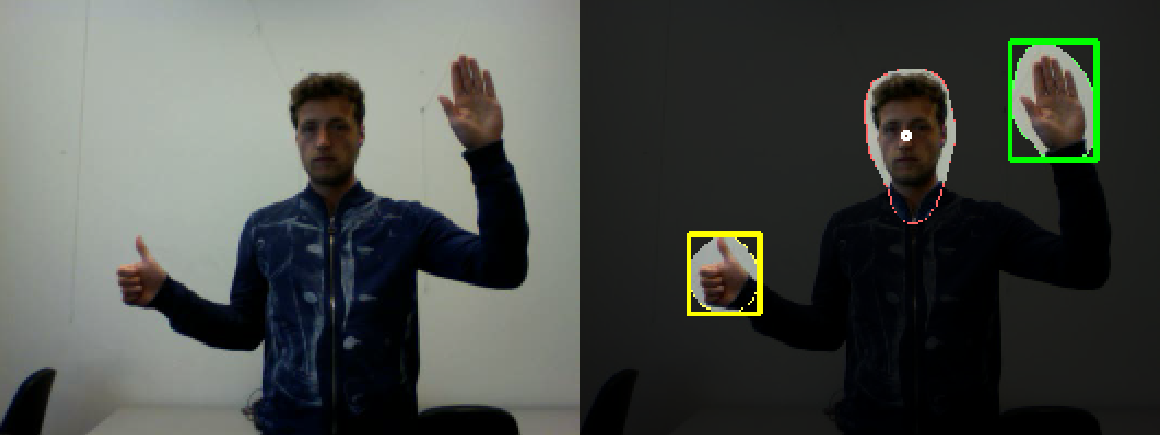
\includegraphics[width=0.8\linewidth]{figures/simple.png}
\caption{Still of movie ivo5 with simple background}
\label{fig:simplebackground}
\end{figure}

\begin{figure}[htbp]
\center{}
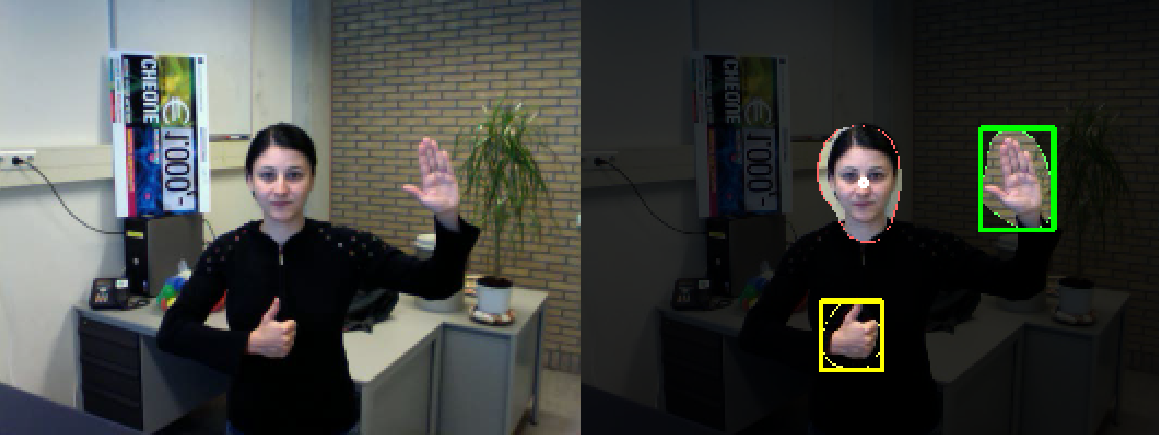
\includegraphics[width=0.8\linewidth]{figures/complex.png}
\caption{Still of movie gosia3 with complex background}
\label{fig:complexbackground}
\end{figure}

\begin{figure}[htbp]
\center{}
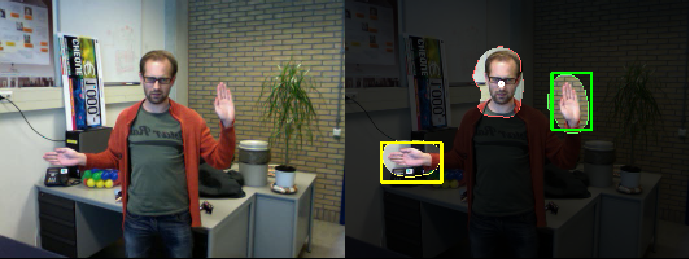
\includegraphics[width=0.8\linewidth]{figures/complexposter.png}
\caption{Still of movie sil1 with complex background with skin like poster}
\label{fig:complexposterbackground}
\end{figure}


\begin{table}
\centering
\begin{tabular}{llll}
\hline\hline
	Test Subject & Movies & Background & Notes \\
\hline
	Anne     & 5 & Simple & None \\
	Arjan    & 5 & Simple & None \\
	Gijs     & 5 & Simple & None \\
	Ivo      & 5 & Simple & None \\
	Jasper 1 & 5 & Simple & None \\
	Peter    & 5 & Simple & None \\
	Hanne    & 5 & Simple & None \\
	Jasper 2 & 3 & Simple & None \\
	Ork      & 3 & Simple & None \\
	Roberto  & 3 & Simple & None \\
	Xiaong   & 3 & Simple & None \\
	Gosia    & 3 & Complex & None \\
	Hamdi    & 3 & Complex & None \\
	Michael  & 3 & Complex & None \\
	Sil      & 3 & Complex + poster & None \\
	Victoria & 3 & Complex + poster & None \\
	Bas      & 3 & Complex + poster & None \\
	Koen     & 3 & Complex + poster & None \\
	Chu      & 3 & Complex + poster & problem with brick wall \\
	Stratos  & 3 & Complex + skin-like colors & problems with white wall \\
\hline
\end{tabular}
\caption{Dataset details}
\end{table}





The dataset is manually labeled. For every sequence of frames where a hand pose is performed a frame number is labeled where the pose resembles the example the most. \autoref{fig:gijs5} is an example of the labeled frames. The train images used to train the classifier where extracted with Sonic Gesture

Usually the 12 Curwen solfege hand symbols are performed in front of the torso as shown in \autoref{fig:hands}. To increase the number of hand poses to be recognized, all 12 Curwen are also performed mirrored next to the body of the recorded subject, see \autoref{fig:hands}. Additionally four extra hand symbols have been added that are not part of the Curwen sequence, see \autoref{fig:hands}. These last four symbols are performed next to the head.

\section{Evaluation}

\subsection{part I - evaluating classifiers}
In this section different evaluators with different parameters are evaluated with changing subsets of the dataset.

\subsubsection{Method}
All hand windows for each symbol in each movie are extracted and the features are extracted and stored. This data in then imported in Matlab, where the experiments are performed. For the SVM classifier the libsvm\footnote{http://www.csie.ntu.edu.tw/~cjlin/libsvm/} package is used. To perform PCA the prtools\footnote{http://www.prtools.org/} package is used. For nearest neighbors the KNN implementation in the biolearning package of matlab itself is used. The evaluation of the classifiers is split out in three runs per classifier:

\paragraph{K-fold per movie using simple dataset only}
here only the movies with a simple background are used. For each run one movie is used for testing and all other movies are used for training. This means for each recorded person currently tested there is also 2 or 4 recordings of him used in the train set. This setting mimics the real life situation where the system is pre-trained with other people than the user but also trained by the user himself, with a simple background.

\paragraph{K-fold per person}
For this evaluation run all movies or used, but per person the movies are used for testing and all other movies for training. Both complex and simple backgrounds are used. This setting mimics the real life situation where the system is pre-trained with only other people than the user of the system, and the background isn't necessarily simple. 

\paragraph{Simple as train set, complex as test set}
As the last evaluation the classifier is trained with all movies with the simple background, and as a test set the movies with the complex background are used. This mimics the real life situation where the training is with recordings in optimal conditions, but the system is used in a complex environment like a living room. Also the system is not trained by the user.

\paragraph{}
For the number of neighbors for K-NN a small number of tests where run, and a value between 3 and 10 for N yielded similar performance. Since a lower number of $k$ can give better performance $k=3$ was used for all experiments.

When PCA was performed on the dataset the smallest eigenvectors where removed so 95\% of the original variance was remaining. On the simple dataset reduce the dimensions from 3780 to 594 dimensions. For the complex set combined with the simple set the dimensionality is reduced to 688 dimensions, for complex only 283 and for the complete dataset 749.

For SVM two kernels are evaluated. The first is the radial basis function (RBF) kernel, since the libsvm documentation states that is a good kernel to use that usually gives good performance. The $c$ and $\gamma$ values for SVM where found by an extensive grid search on the 'per person' tests with only the simple movies performed on a small cluster in the ranges $2.^(-3:2:15)$ for $c$ and $2.^(-15:2:3)$ for $\gamma$. The most optimal values are $\gamma$ = 0.03125. With this $\gamma$ changing the value for $c$ didn't have much effect on the performance, so a value of 64 was taken.

The second kernel used is a precomputed kernel using $\chi^2$.

The Curwen hand symbols that are closely related in a musical scale way are quite similar, for example 'Re' and 'Ri' (\autoref{fig:reri}). It is expected that a lot of misclassifications will be caused by this similarity. To investigate the impact of this issue, 2 different scores are calculated, one for the major scale and one for the full scale. The full scale threats every class as a single class, for the major scale the notes in the major scale and their corresponding similar notes are joined into one class. For example Do an

\begin{figure}[htbp]
  \centering
\subfloat[Re]{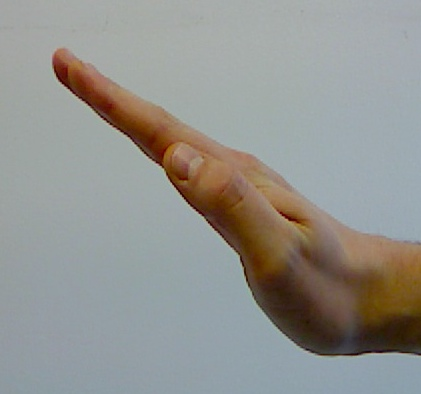
\includegraphics[width=0.2\linewidth,height=0.15\linewidth]{figures/examples/2.jpg}}
\hspace{0.03\linewidth}
\subfloat[Ri]{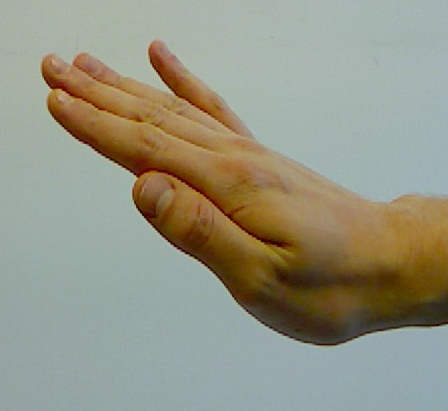
\includegraphics[width=0.2\linewidth,height=0.15\linewidth]{figures/examples/3.jpg}}
  \caption{The hand symbols for Re and Ri}
  \label{fig:reri}
\end{figure}




\subsubsection{Results}

\begin{table}
\centering
\begin{tabular}{lrr}
\hline\hline
Classifier 				&  	Full scale	& Major scale	\\
\hline
KNN3 		&  	84.27\%		& 90.21\%		\\
PCA, KNN3 	& 	83.67\%		& 89.70\%		\\
PCA, SVM RBF ($c=1$ $\gamma=\frac{1}{|features|}$)	& 	76.78\%		& 84.38\%		\\
SVM RBF ($c=2^6$ $\gamma=2^{-5}$) & 86.02\% & 90.88\% \\
PCA, SVM RBF ($c=2^6$ $\gamma=2^{-5}$) &  86.85\% & 91.85\% \\
SVM $\chi^2$ & 87.92\% 		& 91.58\% \\
\hline
\end{tabular}
\caption{k-fold per film using simple dataset only}
\end{table}


\begin{table}
\centering
\begin{tabular}{llrr}
\hline\hline
Dataset & Classifier 				&  	Full scale	& Major scale	\\
\hline
simple set	& KNN3	& 72.93\%, & 82.63\%	\\
simple set	& PCA, SVM RBF ($c=2^6$ $\gamma=2^{-5}$) & 79.71\%, & 86.70\%	\\
full set	& KNN3 & 66.98\%, & 76.32\%	\\
full set	& PCA, KNN3 & 65.31\%, & 76.00\%	\\
full set	& PCA, SVM RBF ($c=1$ $\gamma=\frac{1}{|features|}$) & 64.05\%, & 74.42\%	\\
full set	& PCA, SVM RBF ($c=2^6$ $\gamma=2^{-5}$)& 73.38\%, & 81.44\%	\\
full set    & SVM $\chi^2$ &  71.83\% &80.07\% \\
\hline
\end{tabular}
\caption{k-fold per person}
\end{table}


\begin{table}
\centering
\begin{tabular}{lllcc}
\hline\hline
Descriptors & Classifier 		& pca		&  	Full scale	&	Major scale	\\
\hline
Hog & KNN3				& no	&	58.57\% 	&	72.78\%	\\
Hog & KNN3 				& yes	&	57.62\% 	&	72.17\%	\\
Hog & SVM RBF ($c=2^6$ $\gamma=2^{-5}$)			& yes & 62.14\%	&	73.39\%	\\
Hog & SVM RBF ($c=1$ $\gamma=\frac{1}{|f|}$)	& yes & 55.48\%	&	68.25\%	\\
Hog & SVM $\chi^2$ 		&	yes	&	63.81\%	&	74.71\%	\\
Hog & SVM $\chi^2$		&	yes &	crash 	&	crash \\
\hline
SURF & KNN3				&	no	&	46.19\% 	&	60.17\%	\\
SURF & KNN3										& yes &	44.05\% & 56.65\% \\
SURF & SVM RBF ($c=2^6$ $\gamma=2^{-5}$)		& yes &	44.29\%	&	57.18\%	\\
SURF & SVM RBF ($c=1$ $\gamma=\frac{1}{|f|}$)	& yes &	40.00\%	&	53.28\%	\\
SURF & SVM $\chi^2$								& no  &	37.93\%		&	47.91\%	\\
SURF & SVM $\chi^2$		&	yes	&	crash 	&	crash \\
\hline
\end{tabular}
\caption{simple as trainset, complex as testset. $f$ is the number of features}
\end{table}


full scale accuracy 46.19%
major scale accuracy 60.17%


\begin{figure}[htbp]
\begin{center}
\label{fig:confusion}
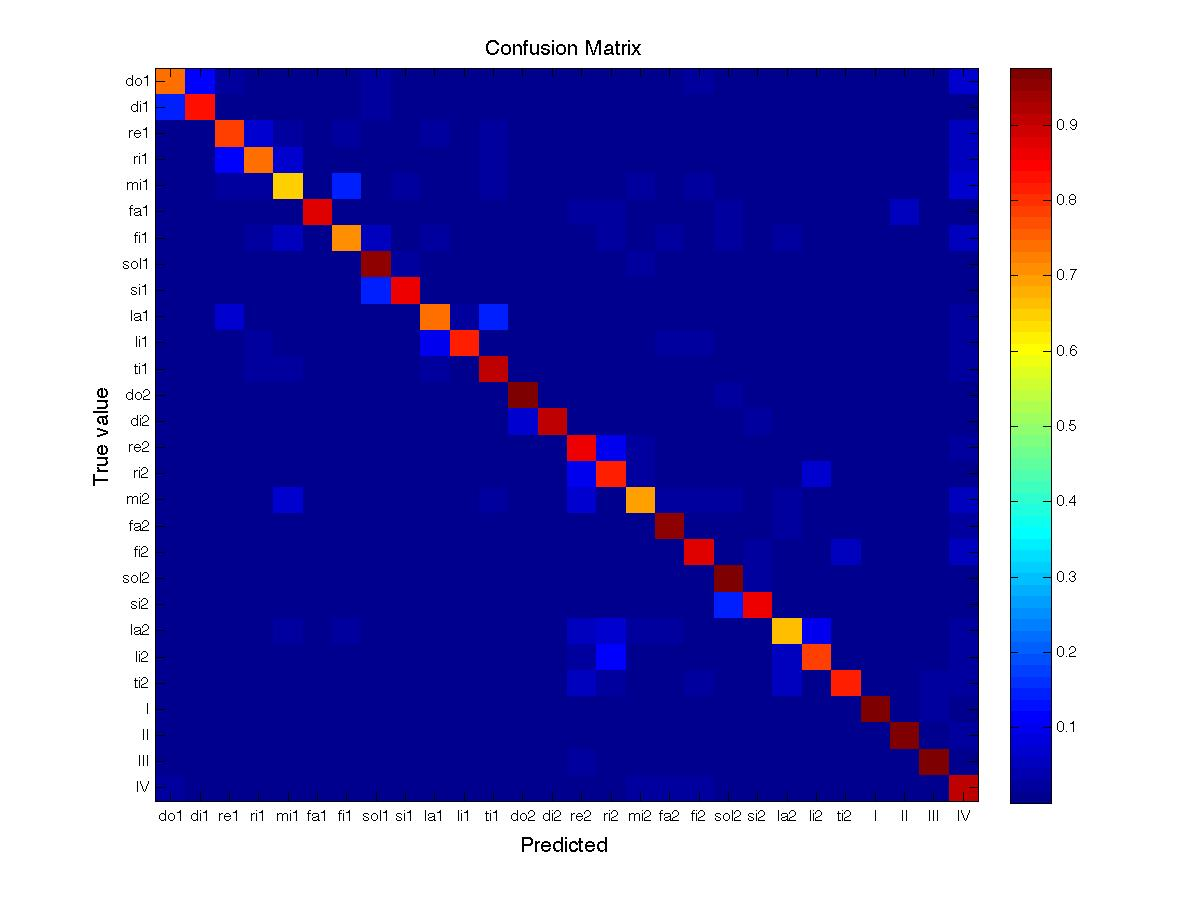
\includegraphics[width=\linewidth]{confmat/confusion.jpg}
\end{center}
\caption{confusion matrix, SVM $\chi^2$, n-fold, per film simple set}
\end{figure}

%>> sum((ones(28,28)-eye(28)).* C)
%6     6     7     6    17     5    14     1     0     3     5     3     3     %1     6    13    10     5     6     5     2     8    10     4     0     0     %1    12



\subsection{Part II - evaluating Sonic Gesture}

\subsubsection{Method}

\begin{figure}[htbp]
\center{}
\subfloat[Without stabilizer]{
	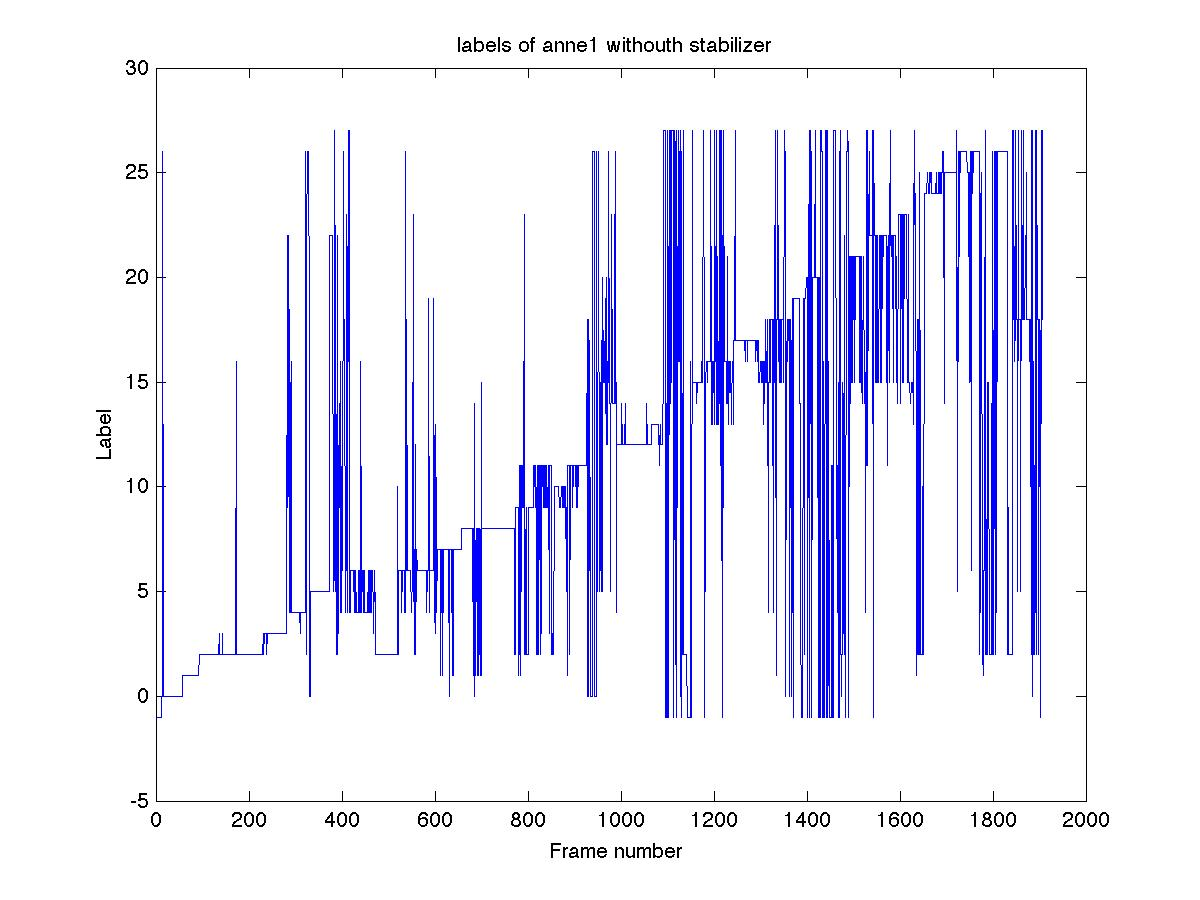
\includegraphics[width=0.3\linewidth]{figures/performance/anne1_unstable.jpg}}
\hspace{0.02\linewidth}
\subfloat[With stabilizer]{
	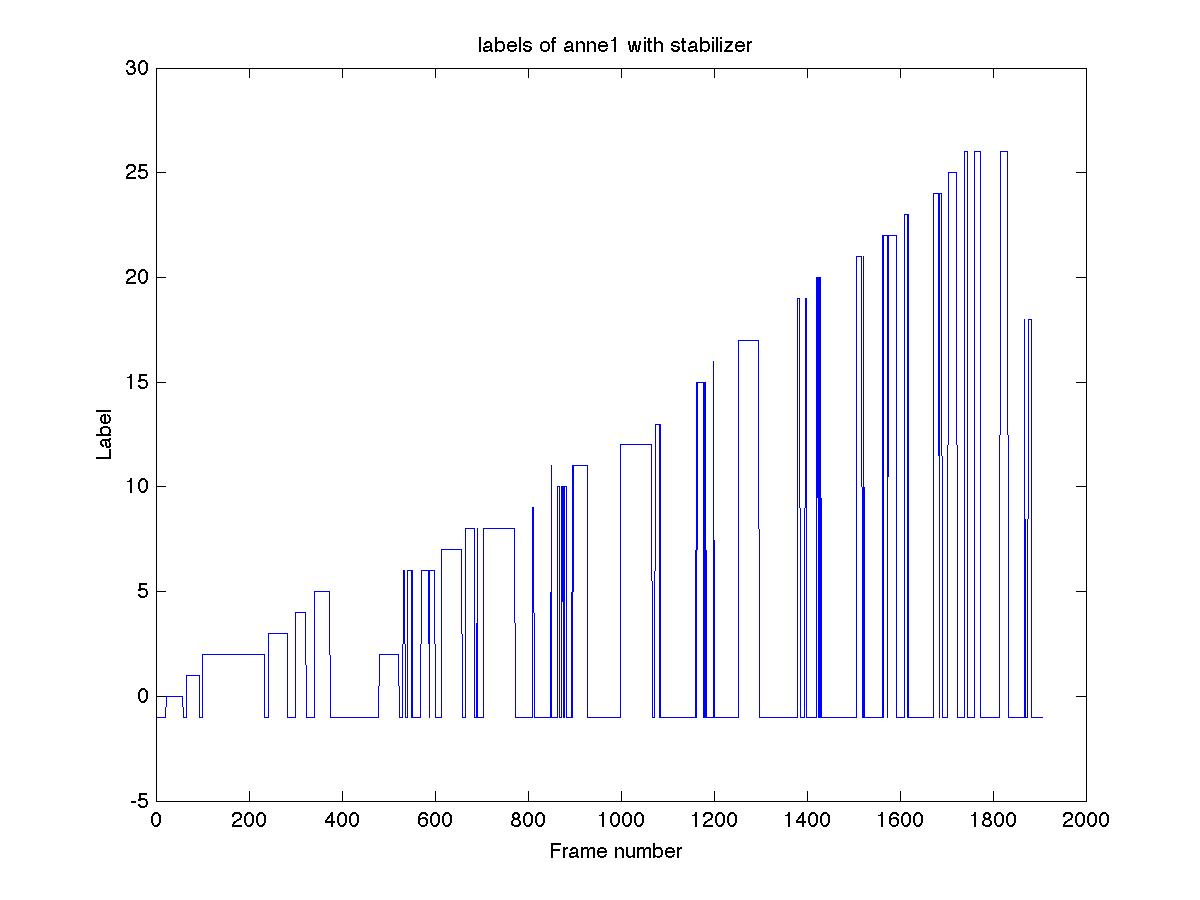
\includegraphics[width=0.3\linewidth]{figures/performance/anne1_stable.jpg}}
\hspace{0.02\linewidth}
\subfloat[Arbitrary movie with stabilizer]{
	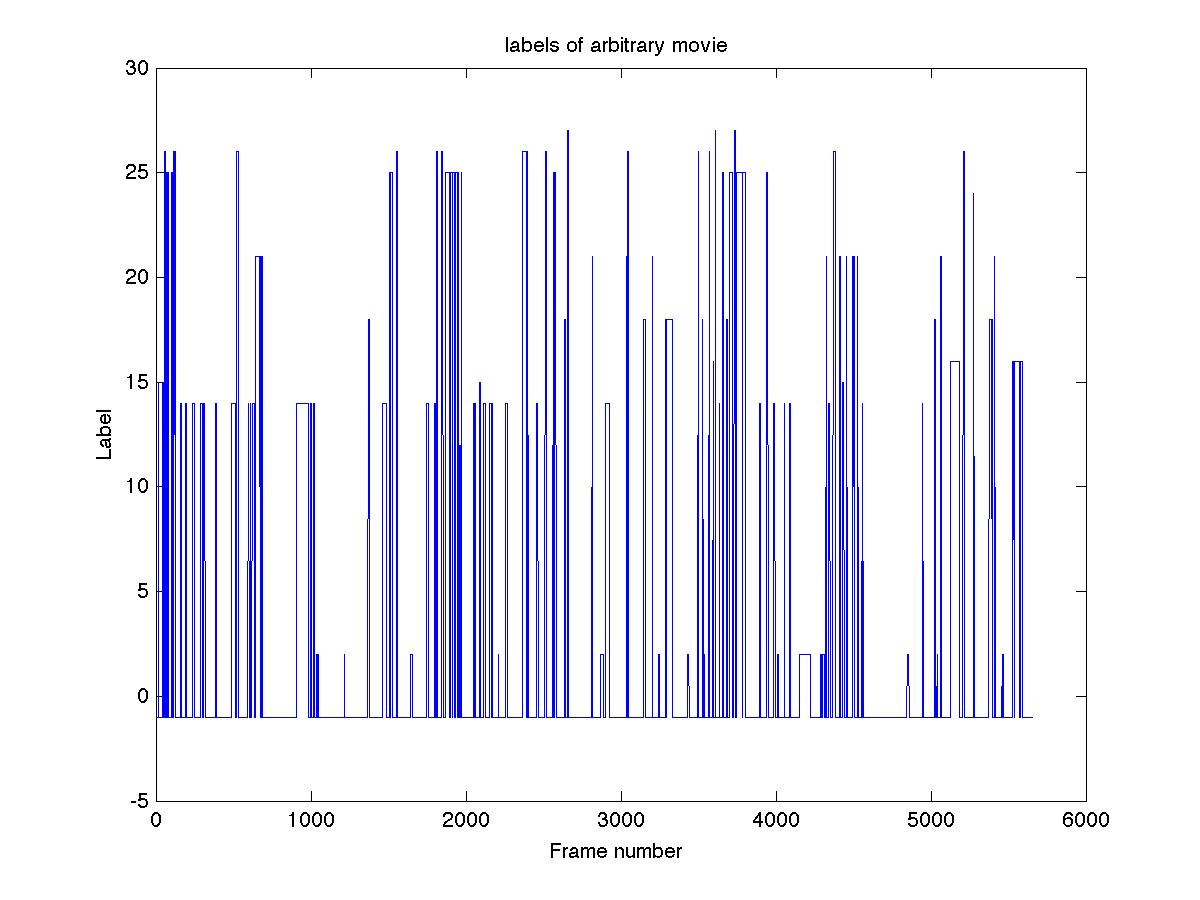
\includegraphics[width=0.3\linewidth]{figures/performance/heilige.jpg}}
\caption{Plots of labels per frame}
\label{fig:performances}
\end{figure}

For this set of experiments the Damerau-Levenshtein distance of a sequence of generated labels to the ground truth is calculated. This value is then divided by the number of labels, 28. A low value is equal to good performance, a high value to bad. The ground truth is a list of incremented integers from 1 to 28. Since some movies are 'poluted' with incorrect hand poses and other people walking through the screen this ground truth isn't really correct. But it is very difficult to impossible to construct a good ground truth in this case, and given the fact that the goal of the recorded movies was to have people perform the 28 hand poses sequentially this is a good alternative. 

\begin{algorithm}
\caption{DamerauLevenshteinDistance(str1, str2)}
\label{dameraulevenshtein}
\begin{algorithmic}
   \REQUIRE a string str1
   \REQUIRE a string str2
   \ENSURE The distance between str1 and str2

   \medskip

   \FOR{$i = 1$ to lenStr1}
       \STATE $\mathbf{D}[i, 0] \Leftarrow i$
   \ENDFOR
   \FOR{$j = 1$ to lenStr2}
       \STATE $\mathbf{D}[0, j] \Leftarrow j$
   \ENDFOR
   \FOR{$i = 1$ to lenStr1}
       \FOR{$j = 1$ to lenStr2}
       		\IF{str1[$i$] $=$ str2[$j$]}
				\STATE cost $\Leftarrow 0$
            \ELSE
				\STATE cost $\Leftarrow 1$
			\ENDIF
			\STATE $x \leftarrow D[i-1, j  ] + 1$ % deletion
			\STATE $y \leftarrow D[i  , j-1] + 1$ % insertion
            \STATE $z \leftarrow D[i-1, j-1] + $ cost % substitution
            \STATE $\mathbf{D}[i, j] \Leftarrow \min(x, y, z)$
            \IF {(str1[$i$] $=$ str2[$j-1$]) $\wedge$ (str1[$i-1$] $=$ str2[$j$])}
				\STATE $\mathbf{D}[i, j] \Leftarrow \min(
                	\mathbf{D}[i, j],
                    \mathbf{D}[i-2, j-2] + $ cost  % transposition
                )
			\ENDIF
		\ENDFOR
	\ENDFOR
   \RETURN d[lenStr1, lenStr2]

\end{algorithmic}
\end{algorithm}
	
\subsubsection{Results}

simple: 0.27 average\\
complex: 0.35 average\\

\begin{table}
\centering
\begin{tabular}{rrrrrrrr}
\hline
name	& 1 & 2 & 3 & 4 & 5 & normalized average & without stabilizer\\
\hline
Anne		&	12.0	&	9.0		&	7.0		&	8.0	&	4.0	&	0.28 & 0.88 \\
Arjan		&	13.0	&	7.0		&	7.0		&	2.0	&	8.0	&	0.26 & 0.83 \\
Gijs		&	4.0		&	5.0		&	6.0		&	6.0	&	4.0	&	0.18 & 0.87 \\
Ivo			&	2.0		&	3.0		&	2.0		&	3.0	&	1.0	&	0.08 & 0.86 \\
Jasper 1	&	19.0	&	13.0	&	6.0		&	6.0	&	12.0 &	0.40 & 0.85 \\
Peter		&	7.0		&	8.0		&	7.0		&	9.0	&	5.0	&	0.26 & 0.86 \\
Hanne		&	9.0		&	0.0		&	1.0		&	7.0	&	2.0	&	0.14 & 0.91 \\
Jasper 2	&	9.0		&	5.0		&	5.0 	& & & 0.23 & 0.90 \\
Ork			&	6.0		&	5.0		&	4.0		& & & 0.18 & 0.86 \\
Roberto		&	19.0	&	8.0		&	13.0	& & & 0.47 & 0.83 \\
Xiaong		&	17.0	&	14.0	&	10.0	& & & 0.49 & 0.88 \\
\hline
Gosia		&	16.0	&	9.0		&	6.0		& & & 0.37 & 0.88 \\
Hamdi		&	14.0	&	12.0	&	15.0	& & & 0.49 & 0.87 \\
Michael		&	6.0		&	8.0		&	13.0	& & & 0.32 & 0.90 \\
Sil			&	14.0	&	17.0	&	13.0	& & & 0.52 & 0.83 \\
Victoria	&	9.0		&	6.0		&	5.0		& & & 0.24 & 0.88 \\
Chu			&	8.0		&	6.0		&	2.0 	& & & 0.19 & 0.89 \\
\hline
Koen		&	11.0	&	9.0		&	11.0 	& & & 0.38 & 0.88\\
Bas			&	15.0	&	12.0	&	9.0		& & & 0.44 & 0.90 \\
Stratos		&	12.0	&	3.0		&	5.0		& & & 0.24 & 0.86 \\

\hline
\end{tabular}
\caption{Damerau-Levenshtein distance of all movies}
\end{table}

\subsection{Part III - Finding Spock}

\subsubsection{Method}
\subsubsection{Results}


\section{Implementation}
\label{sec:implementation}

\begin{figure}[ht]
\begin{center}
\label{fig:sonicgesture}
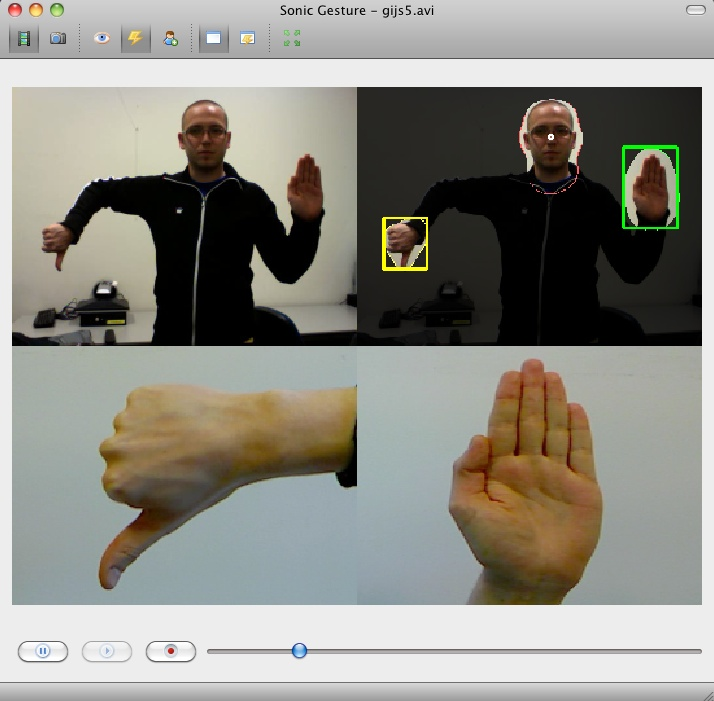
\includegraphics[width=0.6\linewidth]{figures/sonicgesture.jpg}
\end{center}
\caption{screenshot of Sonic Gesture}
\end{figure}

Sonic Gesture has been implemented in C++. Almost all computer vision algorithms used in Sonic Gesture are part of OpenCV, an open source library made for this kind of software. For the graphical interface QT is used. Sonic Gesture has been release as Open Source software and is released under the Apache license. The software can be downloaded, modified and distributed freely from the website\footnote{http://code.google.com/p/sonic-gesture}.

The program can capture directly from a webcam or it can read movies with recorded material. It has 2 modes, one 'finder' mode where hand poses in the video stream are detected. The second mode is the 'capture' mode, which is used to label movies. When labeling a movie in this mode a text file is created with frame positions of the labels. This can later be used to extract the correct frame and extract training data for the classifier. This mode has been used a lot during the gathering of the dataset.

\section{Time performance}
A lot of effort has been put into getting Sonic Gesture as fast as possible. Initially Sonic Gesture was written in Python and used the Python API of OpenCV. Soon it became clear that Python was to limited to do high performance graphic processing so a switch to C++ was made. 

The performance of Sonic Gesture depends on how fast the testing systems CPU power is, if the OpenCV IPP extention is used but also how fast the camera can capture frames. On a Macbook Pro, 2.4 GHz intel core 2 duo with 4 GB of memory using the build-in iSight as camera, processing one frame takes 65 ms on average. This is with the full dataset of 2072 datapoints with 3780 dimensions using the KNN classifier. KNN works fine with low numbers of datapoint, but with high numbers it starts to slow down. Still it is quite fast; around 25 ms on average. SVM will probably perform much faster with a high number of datapoints but we couldn't get the SVM implementation of OpenCV to work. An other expensive operation is the face detection algoritm, when tweaked it takes around 13 ms to locale a face in a image. Since a face position isn't required constantly this is done only every 10th frame, so valuable computation time is saved. An other surprisingly expensive operation is the resizing of a image. Resizing an image to a small size is a crucial part of the pipe line, because some operations on a big image will take too much time. But resizing a image using interpolation is a expensive operation. Where interpolation is not required, for example for rendering on the screen, it is disabled saving more computing time. 



\begin{table}
\centering
\begin{tabular}{cccc}
What & relative time & absolute time & comment \\
\hline
kNN & 37\% & ... & 3780 features, 2016 samples \\
Color space convertion & 8.4\% & ... & \\
Image resizing & 7.6\% & ... & \\
Face detection & 2.3\% & ... &  19\% if every frame \\
\end{tabular}
\caption{Performance timing of Sonic Gesture}
\end{table}

calculating SURF features of a hand train image takes 4ms and results in 11 features on average.



37.9\% KNN
8.4\% color space convertion
7.6\% image resizing
2.3\% haar classifier (19% if not every 10th frame).

\section{Discussion}
As you can see there is a big difference in performance



